\documentclass[12pt, oneside]{article}   	% use "amsart" instead of "article" for AMSLaTeX format
\usepackage{geometry}                		% See geometry.pdf to learn the layout options. There are lots.
\geometry{letterpaper}                   		% ... or a4paper or a5paper or ...
%\geometry{landscape}                		% Activate for rotated page geometry
%\usepackage[parfill]{parskip}    		% Activate to begin paragraphs with an empty line rather than an indent
\usepackage{graphicx}				% Use pdf, png, jpg, or eps§ with pdflatex; use eps in DVI mode
								% TeX will automatically convert eps --> pdf in pdflatex
\usepackage{amssymb}
\usepackage{color}

%SetFonts

%SetFonts

\title{PROVA RISERVATA 2}
\author{2018}
%\date{}							% Activate to display a given date or no date

\begin{document}
\maketitle
%\section{}
%\subsection{}

\begin{figure}[ht!]
\centering
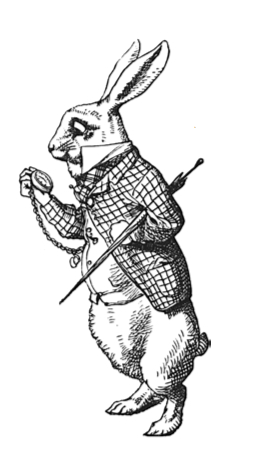
\includegraphics[width=40mm]{cunicio.jpg}
\end{figure}



\section{Regole generali}
La prova riservata \`e destinata esclusivamente agli studenti o studentesse che seguono le lezioni di Analisi Matematica 1 del Professor Enzo Mitidieri durante l'anno accademico 2018/19.  Prove di studenti o studentesse che NON seguono le lezioni non saranno considerate.
  L'ammissione alla prova \`e subordinata alla presenza durante le lezioni.
 Ricordo che la frequenza del corso \`e obbligatoria. La  consegna delle soluzioni deve avvenire {\bf esclusivamente}, {\bf pena l'esclusione},  tramite posta elettronica utilizzando l'indirizzo {\bf proveriservate@gmail.com}.
L'oggetto del messaggio e il nome del file pdf contenente le soluzioni deve essere
\bigskip


{\bf COGNOME  2  2018  }


 \bigskip
{\bf  Messaggi relativi a prove, non conformi a questa richiesta saranno cestinati.}
{\bf Confermare via e-mail all'indirizzo proveriservate@gmail.com la ricezione
di questo file e relativo file sorgente allegato per le soluzioni.}
\section{Regole particolari}
 Il file delle soluzioni deve essere in formato pdf e compilato in ogni sua parte. Pena l'esclusione. Il termine ultimo per la consegna: {\bf Mercoled\`i 26 dicembre 2018 prima delle 18.00}. Il formato del file deve essere {\bf pdf} e compilato in {\bf Tex} o programma equivalente.
Per le soluzioni, utilizzare l'allegato file di sorgente, compilandolo in ogni sua parte. {\bf Prove incomplete di nome, cognome, e matricola  o altre parte da compilare non saranno considerate. Se non avete bonus lasciate in bianco.}
{ \textcolor{red}{\bf Un esercizio si intende svolto se \`e corretto e completo in ogni sua parte. Esercizi con soluzioni parziali non saranno valutati.}}
{\bf  \textcolor{red}{\bf Per essere esonerati dalla prova scritta bisogna raggiungere una valutazione media delle due prove pari a $23/30.$}}

{\bf Consiglio generale. Se non siete in grado di svolgere un esercizio, {\bf NON COPIATE
e NON COLLABORATE CON NESSUNO altrimenti la prova sar\`a annullata.} Consigli sulle soluzioni verranno comunicati
a ricevimento o via SKYPE}. Meglio non svolgere un esercizio piuttosto che copiare.

{\bf Questionario. Inserire qui una foto (formato jpeg o jpg) della valutazione della prima
prova. Inserire i commenti agli esercizi che avete svolto e che vi ho inviato.}





\section{Testo degli esercizi - {\bf \textcolor{red}{Ogni esercizio vale mediamente 10 punti. Un esercizio si intende svolto se \`e corretto e completo in ogni sua parte.
Se un esercizio contiene due parti, per essere considerato completo, \`e necessario svolgere  correttamente e completamente le due parti.}}}
{\bf Esercizio 1}

 Sia $(a_n)$ una successione tale che
$$\lim_{n\to+\infty} a_n= a\neq 0.$$

Provare che la serie
$$\sum_{n=1}^{+\infty} a_{n+1}-a_n, $$

converge assolutamente se e solo se converge assolutamente la serie

$$ \sum_{n=1}^{+\infty} \frac{1}{a_{n+1}} -  \frac{1}{a_{n}}.$$


     {\bf Esercizio 2}
   \bigskip

   i) Sia $f: \mathbb{R_+}\to \mathbb{R}$ una funzione monotona decrescente tale che

    $$\int_0^{+\infty}  f(x)\,dx<+\infty.$$


    Provare che
    $$\lim_{h\to 0^+} \sum_{n=1}^{+\infty} f(nh) = \int_0^{+\infty}  f(x)\,dx.$$

     Utilizzare questo risultato per calcolare

     $$\lim_{h\to 0^+} \sum_{n=1}^{+\infty} \frac{h}{1+h^2 n^2}.$$

     {\bf Suggerimento: Magari a breve... }

   ii) Sia $$f: \mathbb{R_+} \to  \mathbb{R_+}$$

    una funzione positiva e continua tale che,

    $$\int_0^{+\infty}  f(x)\,dx<+\infty.$$

   Dimostrare che
   $$\lim_{n\to +\infty} \frac{1}{n} \int_0^n x\,f(x) \,\,dx =0.$$

   {\bf Suggerimento: Ricordare il teorema di Ces\`aro. }

      {\bf Esercizio 3}
   \bigskip



   Stabilire se la funzione $g: \mathbb{R} \to  \mathbb{R} $ definita da
   $$g(x) : = \sin 3x \, |x|,$$

   \`e uniformemente continua.


\end{document}
